\chapter{Estabilidade Estática Longitudinal e Latero-Direcional}

\section{Cálculo de Estabilidade pelo software AVL}

A análise e o dimensionamento das empenagens realizados no \autoref{estabilidade} foram baseados em métodos semi-empirícos disponíveis em Etkin \cite{etkin1996dynamics}. Com o objetivo de aumentar a fidelidade da análise de estabilidade estática, modelou-se a aeronave no software aberto AVL \cite{avl}. Este programa realiza cálculos aerodinâmicos e de mecânica do voo considerando a aeronave rígida. A configuração da aeronave é uma entrada do programa e o cálculo aerodinâmico é feito utilizando um modelo de vortice lattice para as superfícies sustentadoras.

Os arquivos de geometria e condição de voo utilizados como entrado no programa se encontram no \textbf{Anexo E}. A posição do CG considerada na análise foi a posição mais traseira apresentada no \autoref{passeioCG}. Além disso, a empenagem vertical teve sua área aumentada de $11.89$ para $12.89 m^2$ para aumentar o valor da margem estática lateral. As equações abaixo definem as margens estáticas longitudinal, lateral e direcional respectivamente.

\begin{equation}
  M_{long} = - \frac{\partial C_m}{ \partial \widetilde{C_L}} = - \frac{\frac{\partial C_m}{ \partial \alpha} }{\frac{\partial C_L}{ \partial \alpha} }
\end{equation}

\begin{description}
\item[$M_{long}$  -] Margem estática longitudinal
\item[$h_n$ -] Posição do ponto neutro em relação a CMA
\item[$h$ -] Posição do CG em relação a CMA
\item[$\frac{\partial C_m}{\partial \widetilde{C_L}}$ -] Derivada do momento de arfagem no CG pelo coeficiente de sustentação devido a pertubação
\end{description}

\vspace{1cm}

\begin{equation}
  M_{lat} = - \frac{\partial C_l}{\partial \beta}
\end{equation}

\begin{description}
\item[$M_{lat}$  -] Margem estática lateral
\item[$\frac{\partial C_l}{\partial \beta}$ -] Derivada do momento de rolamento no CG pelo ângulo de derrapagem $\beta$
\end{description}

\vspace{1cm}

\begin{equation}
  M_{dir} = \frac{\partial C_n}{\partial \beta}
\end{equation}

\begin{description}
\item[$M_{dir}$  -] Margem estática direcional
\item[$\frac{\partial C_n}{\partial \beta}$ -] Derivada do momento de guinada no CG pelo ângulo de derrapagem $\beta$
\end{description}

\vspace{1cm}

A \autoref{fig:geom_avl} apresenta a geometria da aeronave utilizada no software AVL.

\begin{figure}[H]
\centering
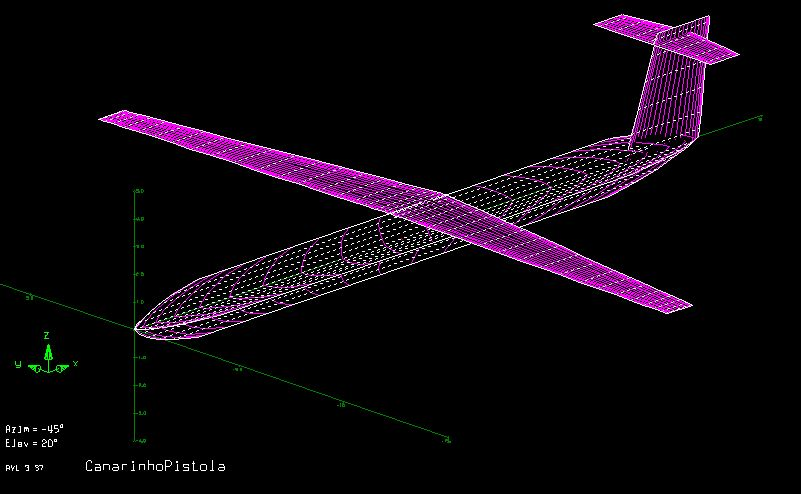
\includegraphics[width=0.8\textwidth]{images/parte4/avl.JPG}
\caption[Geometria da aeronave no AVL]{Geometria da aeronave no AVL}
\label{fig:geom_avl}
\end{figure}

A \autoref{tbl:derivadas_avl} apresenta a estimativa das derivadas realizada com o software AVL no eixo de estabilidade.

\begin{table}[H]
\centering
\begin{tabular}{cccc}
\toprule
$ C_{L_{\alpha}} $ &   6.595 & $ C_{L_{\beta}} $ &     0.0  \\ [0.3cm]
$ C_{Y_{\alpha}} $ &     0.0 & $ C_{Y_{\beta}} $ & -0.6410  \\ [0.3cm]
$ C_{l_{\alpha}} $ &     0.0 & $ C_{l_{\beta}} $ & -0.0449  \\ [0.3cm]
$ C_{m_{\alpha}} $ & -1.2752 & $ C_{m_{\beta}} $ &     0.0  \\ [0.3cm]
$ C_{n_{\alpha}} $ &     0.0 & $ C_{n_{\beta}} $ &  0.1644  \\ [0.3cm]
\bottomrule
\end{tabular}
\begin{tabular}{cccccc}
\toprule
$ C_{L_{p}} $ &     0.0 & $ C_{L_{q}} $ & 14.816  & $ C_{L_{r}} $ &   0.0   \\ [0.3cm]
$ C_{Y_{p}} $ & -0.0895 & $ C_{Y_{q}} $ &    0.0  & $ C_{Y_{r}} $ & 0.6300  \\ [0.3cm]
$ C_{l_{p}} $ & -0.6675 & $ C_{l_{q}} $ &    0.0  & $ C_{l_{r}} $ & 0.0051 \\ [0.3cm]
$ C_{m_{p}} $ &     0.0 & $ C_{m_{q}} $ & -55.95  & $ C_{m_{r}} $ &   0.0  \\ [0.3cm]
$ C_{n_{p}} $ &  0.0404 & $ C_{n_{q}} $ &    0.0  & $ C_{n_{r}} $ & -0.2748 \\ [0.3cm]
\bottomrule
\end{tabular}
\caption[Derivadas da aeronave estimadas pelo AVL]{Derivadas da aeronave estimadas pelo AVL}
\label{tbl:derivadas_avl}
\end{table}

Dessa forma, conclui-se que a aeronave é estável. O controle definido para a aeronave no \autoref{estabilidade} se mantém sendo as dimensões do leme de direção e aileron identicas à aeronave ATR 42-600.

\section{Estabilidade para CG alternativo (sem APU)}

Para a configuração da aeronave sem APU, a posição mais traseira do CG é
\begin{equation}
  x_{CG} = 12,82\text{m}
\end{equation}
Isso é bem próximo da posição nominal do CG, a 12,9m do nariz.
 Dessa forma, a estabilidade não é muito afetada.
 A aeronave continua estável.
 As derivadas aerodinâmicas para essa configuração são:

\begin{table}[H]
\centering
\caption{Derivadas aerodinâmicas para posição alternativa do CG (sem APU)}
\begin{tabular}{cccc}
\toprule
$ C_{L_{\alpha}} $ &   6.607 & $ C_{L_{\beta}} $ &     0.0  \\ [0.3cm]
$ C_{Y_{\alpha}} $ &     0.0 & $ C_{Y_{\beta}} $ & -0.6384  \\ [0.3cm]
$ C_{l_{\alpha}} $ &     0.0 & $ C_{l_{\beta}} $ & -0.0433  \\ [0.3cm]
$ C_{m_{\alpha}} $ & -1.2882 & $ C_{m_{\beta}} $ &     0.0  \\ [0.3cm]
$ C_{n_{\alpha}} $ &     0.0 & $ C_{n_{\beta}} $ &  0.1628  \\ [0.3cm]
\bottomrule
\end{tabular}
\begin{tabular}{cccccc}
\toprule
$ C_{L_{p}} $ &     0.0 & $ C_{L_{q}} $ & 14.1248  & $ C_{L_{r}} $ &   0.0   \\ [0.3cm]
$ C_{Y_{p}} $ & -0.0534 & $ C_{Y_{q}} $ &    0.0  & $ C_{Y_{r}} $ & 0.6300  \\ [0.3cm]
$ C_{l_{p}} $ & -0.6656 & $ C_{l_{q}} $ &    0.0  & $ C_{l_{r}} $ & 0.0051 \\ [0.3cm]
$ C_{m_{p}} $ &     0.0 & $ C_{m_{q}} $ & -55.6492  & $ C_{m_{r}} $ &   0.0  \\ [0.3cm]
$ C_{n_{p}} $ &  0.0142 & $ C_{n_{q}} $ &    0.0  & $ C_{n_{r}} $ & -0.2748 \\ [0.3cm]
\bottomrule
\end{tabular}
\end{table}